\PassOptionsToPackage{unicode=true}{hyperref} % options for packages loaded elsewhere
\PassOptionsToPackage{hyphens}{url}
%
\documentclass[]{article}
\usepackage{lmodern}
\usepackage{amssymb,amsmath}
\usepackage{ifxetex,ifluatex}
\usepackage{fixltx2e} % provides \textsubscript
\ifnum 0\ifxetex 1\fi\ifluatex 1\fi=0 % if pdftex
  \usepackage[T1]{fontenc}
  \usepackage[utf8]{inputenc}
  \usepackage{textcomp} % provides euro and other symbols
\else % if luatex or xelatex
  \usepackage{unicode-math}
  \defaultfontfeatures{Ligatures=TeX,Scale=MatchLowercase}
\fi
% use upquote if available, for straight quotes in verbatim environments
\IfFileExists{upquote.sty}{\usepackage{upquote}}{}
% use microtype if available
\IfFileExists{microtype.sty}{%
\usepackage[]{microtype}
\UseMicrotypeSet[protrusion]{basicmath} % disable protrusion for tt fonts
}{}
\IfFileExists{parskip.sty}{%
\usepackage{parskip}
}{% else
\setlength{\parindent}{0pt}
\setlength{\parskip}{6pt plus 2pt minus 1pt}
}
\usepackage{hyperref}
\hypersetup{
            pdfborder={0 0 0},
            breaklinks=true}
\urlstyle{same}  % don't use monospace font for urls
\usepackage[margin=1in]{geometry}
\usepackage{graphicx,grffile}
\makeatletter
\def\maxwidth{\ifdim\Gin@nat@width>\linewidth\linewidth\else\Gin@nat@width\fi}
\def\maxheight{\ifdim\Gin@nat@height>\textheight\textheight\else\Gin@nat@height\fi}
\makeatother
% Scale images if necessary, so that they will not overflow the page
% margins by default, and it is still possible to overwrite the defaults
% using explicit options in \includegraphics[width, height, ...]{}
\setkeys{Gin}{width=\maxwidth,height=\maxheight,keepaspectratio}
\setlength{\emergencystretch}{3em}  % prevent overfull lines
\providecommand{\tightlist}{%
  \setlength{\itemsep}{0pt}\setlength{\parskip}{0pt}}
\setcounter{secnumdepth}{0}
% Redefines (sub)paragraphs to behave more like sections
\ifx\paragraph\undefined\else
\let\oldparagraph\paragraph
\renewcommand{\paragraph}[1]{\oldparagraph{#1}\mbox{}}
\fi
\ifx\subparagraph\undefined\else
\let\oldsubparagraph\subparagraph
\renewcommand{\subparagraph}[1]{\oldsubparagraph{#1}\mbox{}}
\fi

% set default figure placement to htbp
\makeatletter
\def\fps@figure{htbp}
\makeatother

\usepackage{ctex}
\setmainfont{STHeitiSC-Medium}
\setCJKmainfont{STHeitiSC-Medium}
\usepackage{xcolor}
\usepackage{fancyhdr}
\pagestyle{plain}
\usepackage{sectsty}
\definecolor{glaucous}{rgb}{0.38, 0.51, 0.71}
\definecolor{lavenderblush}{rgb}{1.0, 0.94, 0.96}
\definecolor{grey}{RGB}{96, 96, 96}
\usepackage{enumitem}% http://ctan.org/pkg/enumitem
\usepackage[empty]{fullpage}% http://ctan.org/pkg/fullpage
\usepackage{color}% http://ctan.org/pkg/color
\usepackage{hyperref}% http://ctan.org/pkg/hyperref
\usepackage{geometry}
\geometry{papersize={15.5cm,50cm},left=0.5cm,right=0.5cm,top=0.3cm,bottom=0.3cm}
\usepackage{blindtext}
\usepackage[center]{caption}
\usepackage[font=Large]{caption}
\usepackage{subfigure}
\usepackage{float}
\usepackage{graphicx}
\usepackage{booktabs}
\usepackage[justification=centering]{caption}
\usepackage{threeparttable}
\usepackage{longtable}
\usepackage{array}
\usepackage{multirow}
\usepackage{wrapfig}
\usepackage{float}
\usepackage{colortbl}
\usepackage{pdflscape}
\usepackage{tabu}
\usepackage{threeparttable}
\usepackage{threeparttablex}
\usepackage[normalem]{ulem}
\usepackage{makecell}
\usepackage{xcolor}
\linespread{1.85}
\setlength{\parskip}{1em}
\setlength{\footskip}{20pt}
\usepackage{booktabs}
\usepackage{longtable}
\usepackage{array}
\usepackage{multirow}
\usepackage{wrapfig}
\usepackage{float}
\usepackage{colortbl}
\usepackage{pdflscape}
\usepackage{tabu}
\usepackage{threeparttable}
\usepackage{threeparttablex}
\usepackage[normalem]{ulem}
\usepackage{makecell}
\usepackage{xcolor}

\author{}
\date{\vspace{-2.5em}}

\begin{document}

\captionsetup[figure]{name={图},labelsep=space}
\captionsetup[table]{name={表},labelsep=space} 
\fontsize{22}{22}
\selectfont
\vspace{-10truemm}

\newcommand{\resheading}[1]{%
  \noindent\fcolorbox{lavenderblush}{lavenderblush}{\makebox[\dimexpr\textwidth-2\fboxsep-2\fboxrule][c]{\textbf{~#1}}}%
}

\begin{center}

\includegraphics[height=2cm]{./input/logo2.png} 
\end{center}

\begin{center}
\fontsize{45}{45}
\textcolor{glaucous}{\textbf{新冠早报}}
\end{center}

\begin{center}
\fontsize{22}{22}
{\textcolor{glaucous}{\textbf{第72期 \space 6月30日}}}
\end{center}

\vspace{2mm}
\begin{center}

\includegraphics[height=2cm]{./input/title1.png} 
\end{center}

\vspace{-5mm}

\begin{huge}{\textcolor{glaucous}{\textbf{国际}}}\end{huge}

\vspace{-3mm}

\begin{center}
\textcolor{glaucous}{英国广播公司 (BBC)}\\特朗普取消留学生驱逐出境计划
\end{center}

当地时间7月14日,美国总统唐纳德·特朗普政府宣布放弃于上周颁布的一项针对在美留学生的计划。该计划规定,对于申请今年秋季入学的留学生,如果学校受疫情影响仅开设网课,学生将无法获得签证;而对于已经在美国境内的留学生,如果仅选择网课,则必须离境或转学至提供面授课的学校,否则将可能被驱逐出境。哈佛大学和麻省理工学院曾对该计划提起诉讼。

\begin{center}
\textcolor{glaucous}{有线电视新闻网 (CNN)}\\美国疾控中心称 “若无疫苗控制,疫情或将持续几年”
\end{center}

当地时间7月14日,美国疾病预防控制中心(CDC)主任罗伯特·雷德菲尔德在与巴克研究所共同举行的网络研讨会上说,如果没有诸如疫苗之类的``生物对策'',我们将不得不花费两三年的时间来与新冠病毒作斗争。雷德菲尔德还表示,希望在明年一月前获得成功的疫苗,从而保护美国公众免受新冠病毒侵害。

\begin{center}
\textcolor{glaucous}{华盛顿邮报 (Washington Post)}\\实验性新冠病毒疫苗首次人体试验结果证明安全
\end{center}

根据《新英格兰医学杂志》7月14日发表的一篇文章,由生物技术公司Moderna和美国国家过敏与传染病研究所开发的一种实验性新冠病毒疫苗是安全的,并在全部45名参与者的首次人体测试中引发了免疫反应。Moderna于同日宣布将从7月27日起面向三万人进行第三阶段试验,以进一步检测该疫苗的有效性和安全性。

\begin{center}
\textcolor{glaucous}{中新网}\\比利时专家警告:欧洲已出现第二波新冠肺炎疫情
\end{center}

据比利时《布鲁塞尔时报》当地时间7月14日消息,比利时流行病学家皮埃尔·范·达姆表示,欧洲地区已经出现第二波新冠肺炎疫情,他担心欧洲已失去了对新冠病毒的控制。达姆认为,疫情再次反弹与实施解禁措施太快有关,为此,``各方必须采取非常严格的措施,否则欧洲将很快失去赢得的一切''。达姆还建议比利时卫生部门继续公布该国每日的新增新冠肺炎确诊病例数据,而不是公布七日的平均数,因为每日数据对于公众而言是一个重要信号,可使公众更好地了解当地情况。

\begin{center}
\textcolor{glaucous}{有线电视新闻网 (CNN)}\\法国研究发现新冠病毒可通过胎盘传播
\end{center}

当地时间7月14日,一份发表在《自然通讯》杂志上的报告显示,母亲在怀孕的最后三个月被感染新冠病毒后,新生儿的新冠病毒检测也呈阳性。从胎盘中检测到的新冠病毒载量比母亲或新生儿的血液、胎儿出生前羊水中的病毒载量高得多。法国研究团队由此推断,新冠病毒穿过胎盘并感染了子宫中的婴儿。

\begin{center}
\textcolor{glaucous}{有线电视新闻网 (CNN)}巴西总统宣布免征549项抗疫物资进口关税
\end{center}

当地时间7月14日,巴西总统贾尔·博尔索纳罗宣布取消用于抗击新冠疫情的34种医疗物资(包括伊维菌素、一次性呼吸防护口罩生产和包装机械等)的进口关税。博尔索纳罗说,目前巴西共有549种抗疫药品、设备和器材等免除进口关税。该决议临时将抗疫物资关税减至进口税率的百分之零,来对抗新冠大流行。

\vspace{5mm}

\begin{huge}{\textcolor{glaucous}{\textbf {国内}}}\end{huge}

\vspace{-3mm}

\begin{center}
\textcolor{glaucous}{央视新闻}\\国家卫健委:院前医疗急救环节由专车执行高风险任务
\end{center}

国家卫健委7月13日公开发布通知,提出专门车组执行高风险任务,在调度环节加强问询,最大程度降低转运过程中的传播风险和医患交叉感染风险。通知要求,各地卫生健康行政部门统筹负责辖区内新冠肺炎病例的转运指挥调度工作,划拨一定数量的负压救护车辆和专业人员,成立新冠肺炎疫情转运车组,采取平战结合管理,``战时''全力承担新冠肺炎疑似病例、确诊病例、无症状感染者以及发热相关病例的转运任务,平时承担日常院前医疗急救任务。

\vspace{10mm}

\begin{center}

\includegraphics[height=2cm]{./input/title2.png} 
\end{center}

\begin{Large}
\vspace{-7mm}
{数据源:约翰霍普金斯大学,The COVID Tracking  Project}
\end{Large}

\vspace{-7mm}

\begin{Large}
{数据截止至:北京时间6月30日 上午8:00}
\end{Large}

\begin{huge}{\textcolor{glaucous}{\textbf {一、世界疫情}}}\end{huge}

\(\bullet\)截止昨日,全球累计确诊病例达13,102,954例,累计死亡573,036例。共有22个国家累计确诊病例数超过10万例,其中7个为亚洲国家,6个为欧洲国家,8个为美洲国家,另有1个非洲国家。

\(\quad\)\(\diamond\)北美洲地区确诊病例数持高不下,截止至昨日,累计确诊病例数已接近400万例,依旧排名第一。

\(\quad\)\(\diamond\)南美洲和亚洲确诊病例数持续增长,截止至昨日,确诊病例数均接近300万例。

\begin{figure}[H]
\captionsetup{font={huge}}
\caption{世界疫情分布趋势图\\ \vspace{-3mm}(来源:WHO)} %最终文档中希望显示的图片标题
\centering
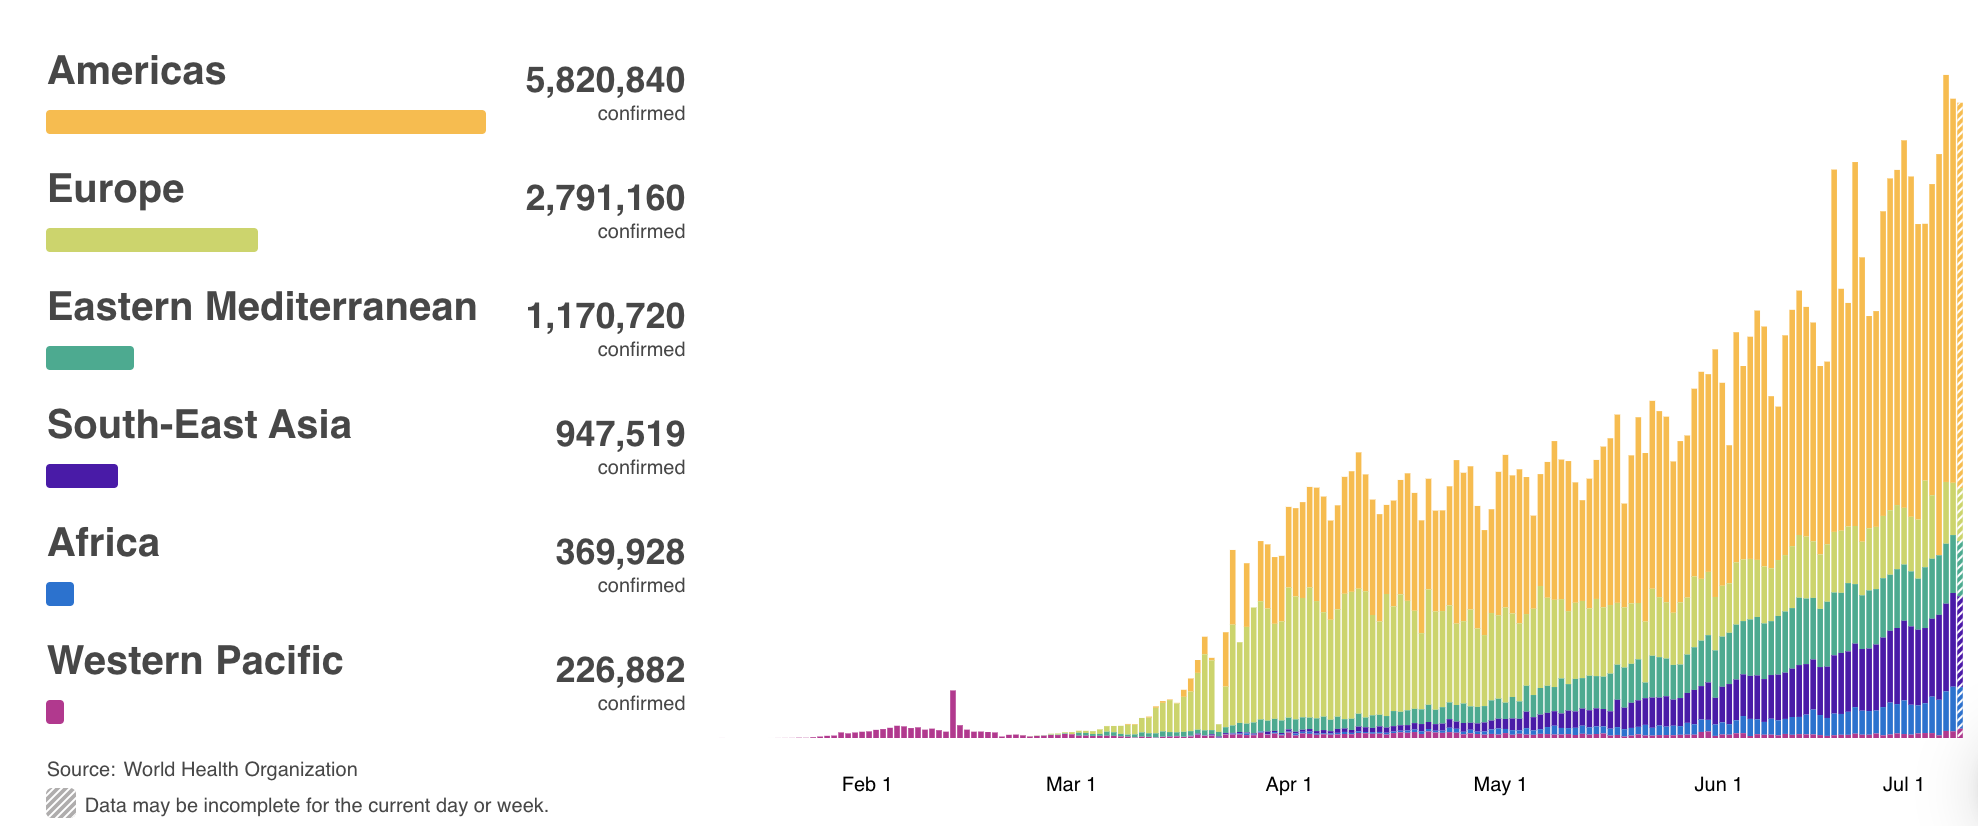
\includegraphics[]{./input/covid1.png} %插入图片,[]中设置图片大小,{}中是图片文件名
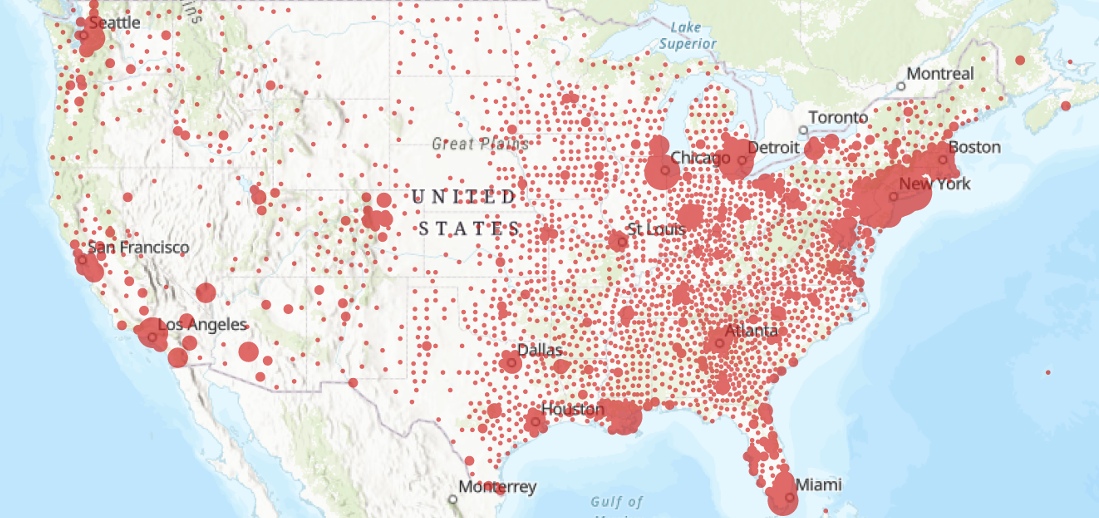
\includegraphics[]{./input/covid4.png}
\label{} %用于文内引用的标签
\end{figure}

\begin{table}[H]
    \centering \begin{table}[H]
\centering\begingroup\fontsize{20}{22}\selectfont

\resizebox{\linewidth}{!}{
\begin{tabular}{rlrrrr}
\toprule
\multicolumn{0}{c}{\textbf{ }} & \multicolumn{5}{c}{\textbf{表1 累计确诊前十位国家}} \\
  & 国家(地区) & 累计确诊 & 粗发病率* & 累计死亡 & 病死率\%\\
\midrule
\rowcolor{gray!6}  1 & 美国 US & 3,363,056 & 1,016 & 135,605 & 4.0\\
2 & 巴西 Brazil & 1,884,967 & 887 & 72,833 & 3.9\\
\rowcolor{gray!6}  3 & 印度 India & 906,752 & 66 & 23,727 & 2.6\\
4 & 俄罗斯 Russia & 732,547 & 502 & 11,422 & 1.6\\
\rowcolor{gray!6}  5 & 秘鲁 Peru & 330,123 & 1,001 & 12,054 & 3.7\\
6 & 智利 Chile & 317,657 & 1,662 & 7,024 & 2.2\\
\rowcolor{gray!6}  7 & 墨西哥 Mexico & 304,435 & 236 & 35,491 & 11.7\\
8 & 英国 UK & 291,691 & 430 & 44,915 & 15.4\\
\rowcolor{gray!6}  9 & 南非 South Africa & 287,796 & 485 & 4,172 & 1.4\\
10 & 伊朗 Iran & 259,652 & 309 & 13,032 & 5.0\\
\bottomrule
\end{tabular}}
\endgroup{}
\end{table} \begin{tablenotes}
        \fontsize{12}{12}
        \selectfont
        \item 注:*粗发病率定义:在一定时间内,特定范围人群中某病新发生的病例出现的频率。计算方式:(累计确诊病例/人口)×10万;
      \end{tablenotes}
    \end{table}

\(\bullet\)全球昨日新增确诊接近20万例(192,928例),新增死亡3,914例(表2)。

\(\quad\)\(\diamond\)北美洲昨日新增确诊接近6.8万例,新增死亡974例。其中虽然美国近两天新增病例数较前几日略有下降,但依旧占北美洲日新增确诊数的85\%以上。

\(\quad\)\(\diamond\)南美洲昨日新增确诊超过3.6万例,新增死亡超过1,300例。其中虽然巴西近两日新增病例和死亡病例数较前一周有明显下降,但仍占南美洲日新增和死亡病例的55\%以上。此外,该地区日新增第二的国家哥伦比亚近期日新增波动明显,自上周六达到近两周最高峰(6,587)后,周日日新增有小幅度下降。

\(\quad\)\(\diamond\)亚洲昨日新增确诊近5.6万例,新增死亡1,137例。超过一半日新增病例来自于印度。值得注意的是,伊朗昨日日新增死亡病例数首次超过200例,成为该地区排名第二、世界排名第四的国家,显示该国家医疗资源面临一定压力。

\(\quad\)\(\diamond\)非洲昨日新增确诊超过1.6万例,新增死亡218例。南非疫情持续扩散,近五天单日新增确诊病例均在12,000例上下波动。

\begin{table}[H]
    \centering \begin{table}[H]
\centering\begingroup\fontsize{20}{22}\selectfont

\begin{tabular}{rlrr}
\toprule
\multicolumn{0}{c}{\textbf{ }} & \multicolumn{2}{c}{\textbf{表2 日新增病例前十位国家}} \\
  & 国家 & 新增确诊 & 新增死亡\\
\midrule
\rowcolor{gray!6}  1 & 美国 US & 58,114 & 400\\
2 & 印度 India & 28,498 & 553\\
\rowcolor{gray!6}  3 & 巴西 Brazil & 20,286 & 733\\
4 & 南非 South Africa & 11,554 & 93\\
\rowcolor{gray!6}  5 & 俄罗斯 Russia & 6,511 & 104\\
6 & 哥伦比亚 Colombia & 5,083 & 208\\
\rowcolor{gray!6}  7 & 墨西哥 Mexico & 4,685 & 485\\
8 & 秘鲁 Peru & 3,797 & 184\\
\rowcolor{gray!6}  9 & 哈萨克斯坦 Kazakhstan & 3,502 & 0\\
10 & 阿根廷 Argentina & 3,099 & 58\\
\bottomrule
\end{tabular}
\endgroup{}
\end{table} \end{table}
\vspace{5mm}
\begin{figure}[H]
\centering
\captionsetup{font={huge}}
\caption{日新增确诊病例国家趋势图}
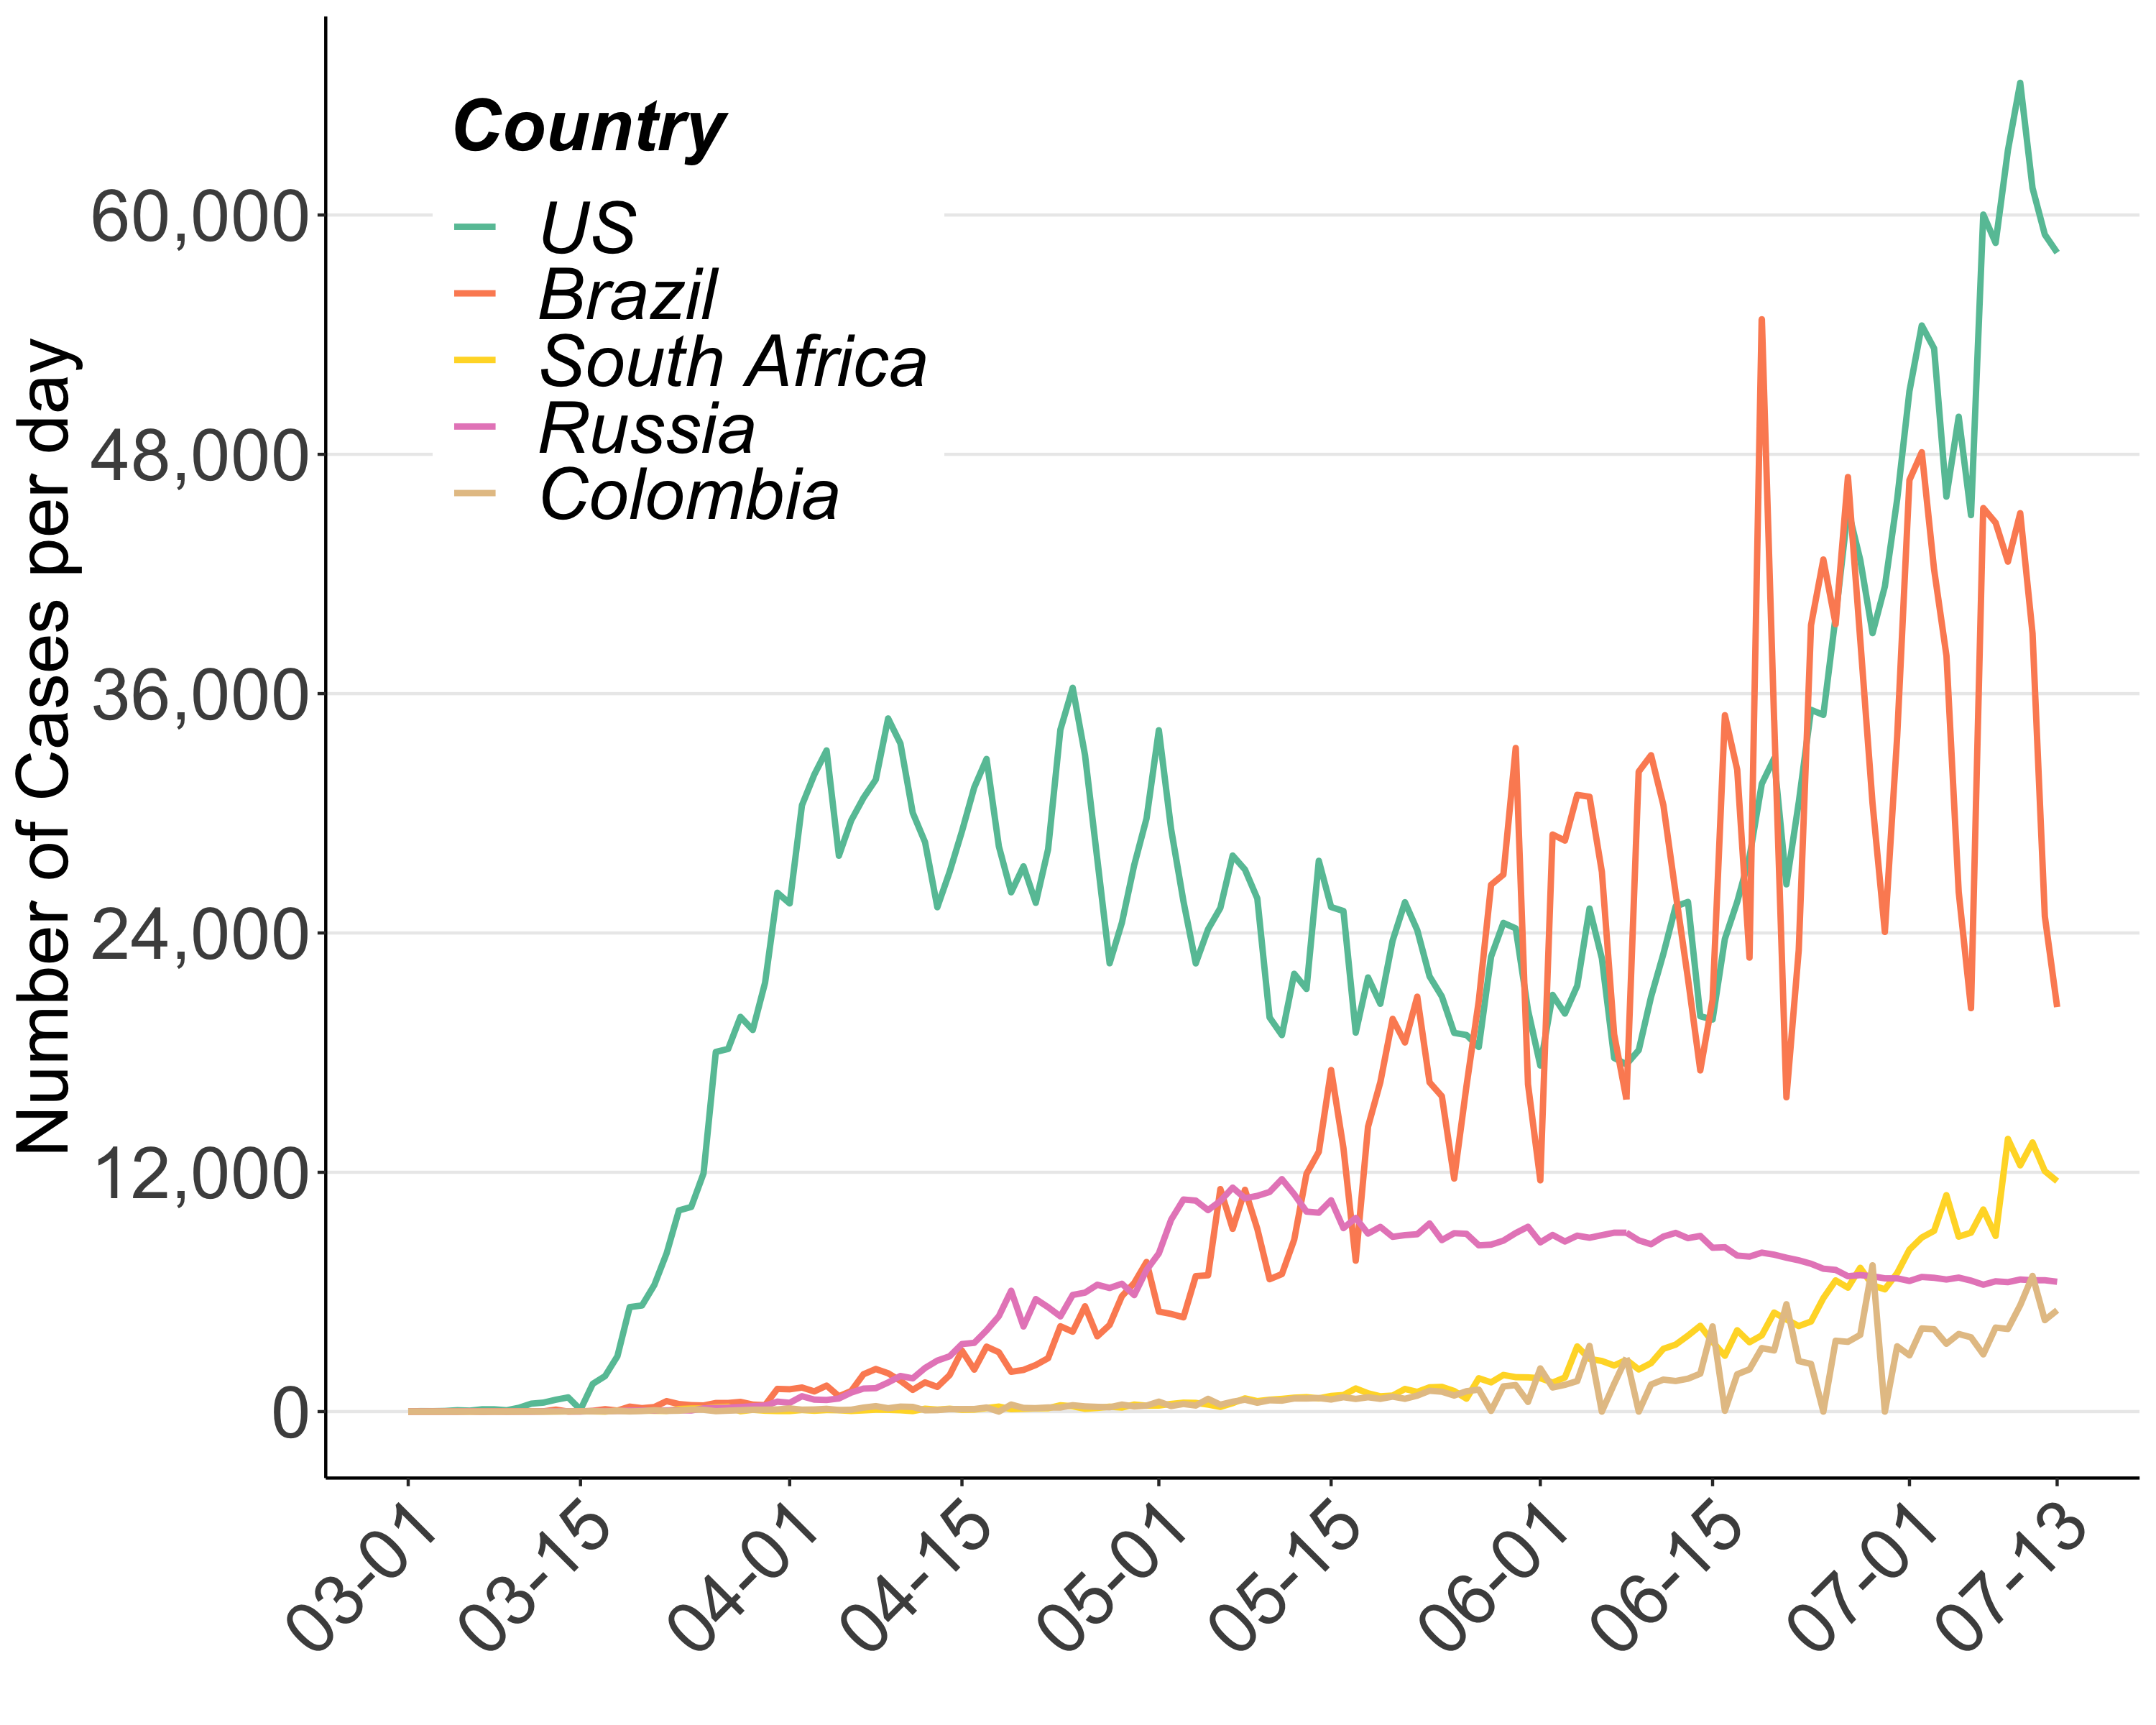
\includegraphics[]{./input/covid2.png}
\end{figure}

\begin{figure}[H]
\centering
\captionsetup{font={huge}}
\caption{日新增死亡病例国家趋势图}
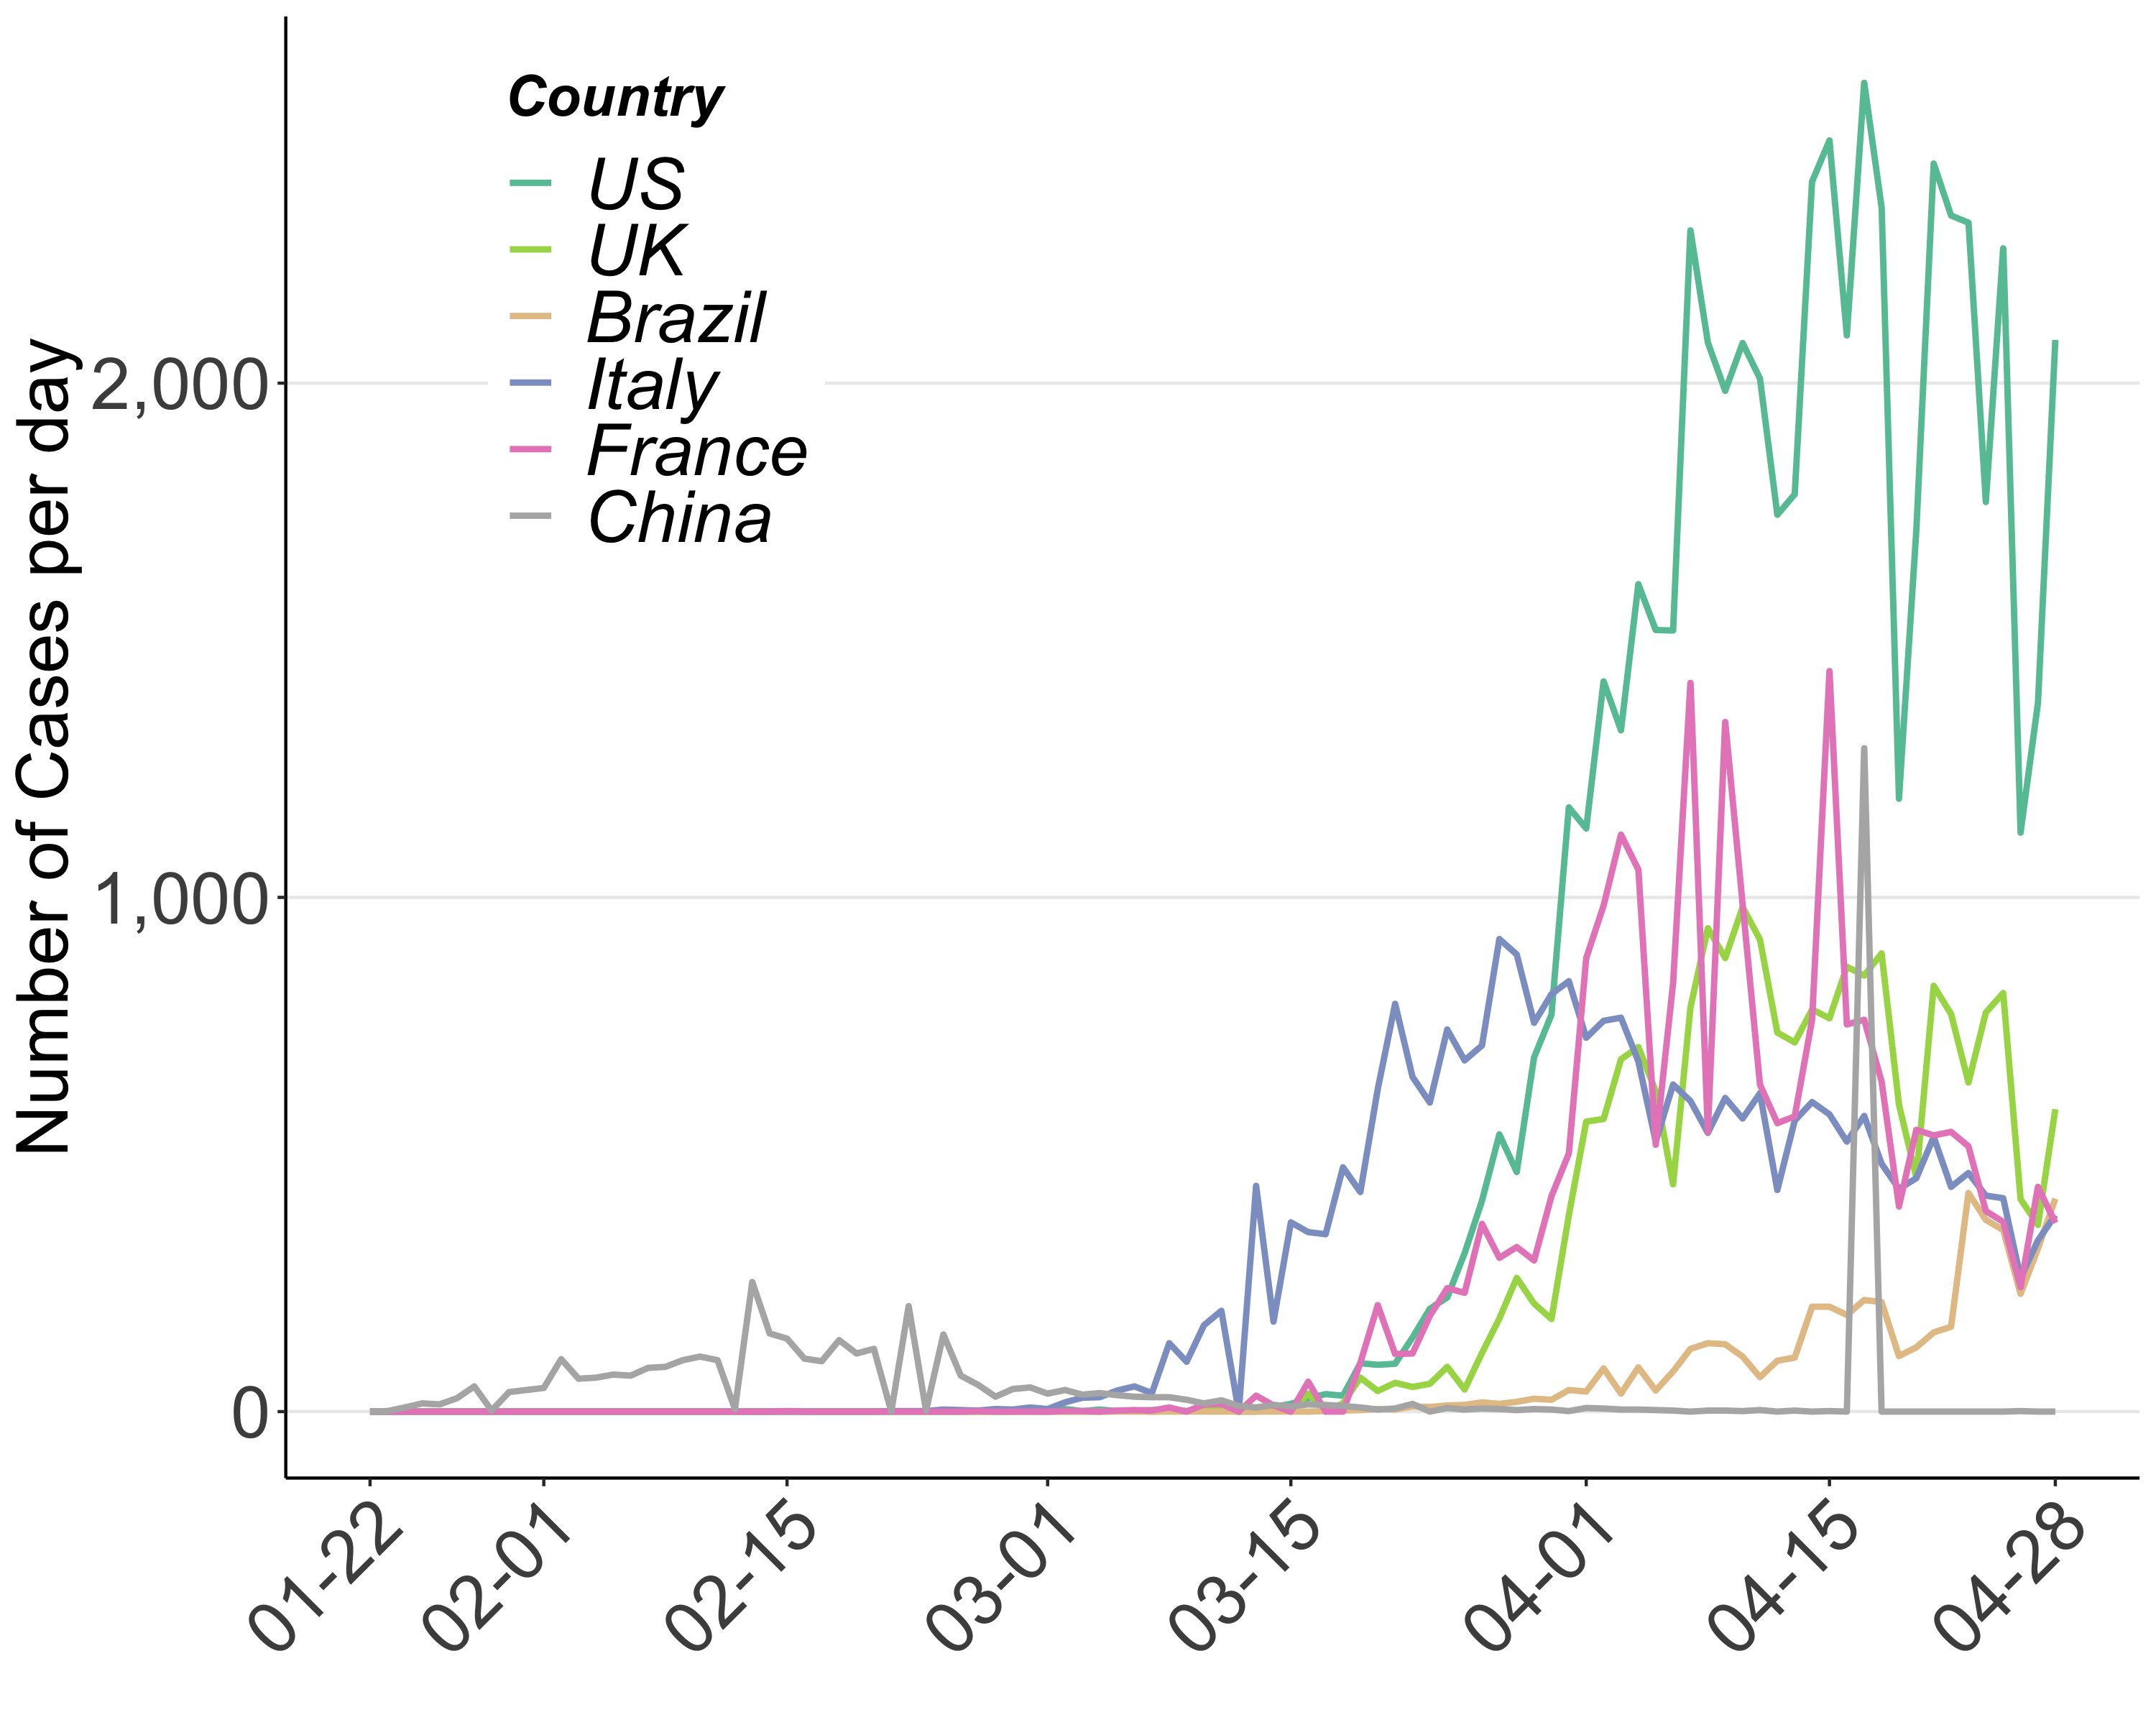
\includegraphics[]{./input/covid3.png}
\end{figure}

\vspace{-7mm}

\begin{huge}{\textcolor{glaucous}{\textbf {二、美国疫情}}}\end{huge}

\(\bullet\)截至昨日,
美国累计确诊病例数为3,363,056例,累计死亡135,605例。

\(\quad\)\(\diamond\)共有42个州及地区累计确诊病例超过1万例,20个州累计确诊病例超过5万例。

\begin{figure}[H]
\centering
\captionsetup{font={huge}}
\caption{美国日新增确诊前五位州趋势图}
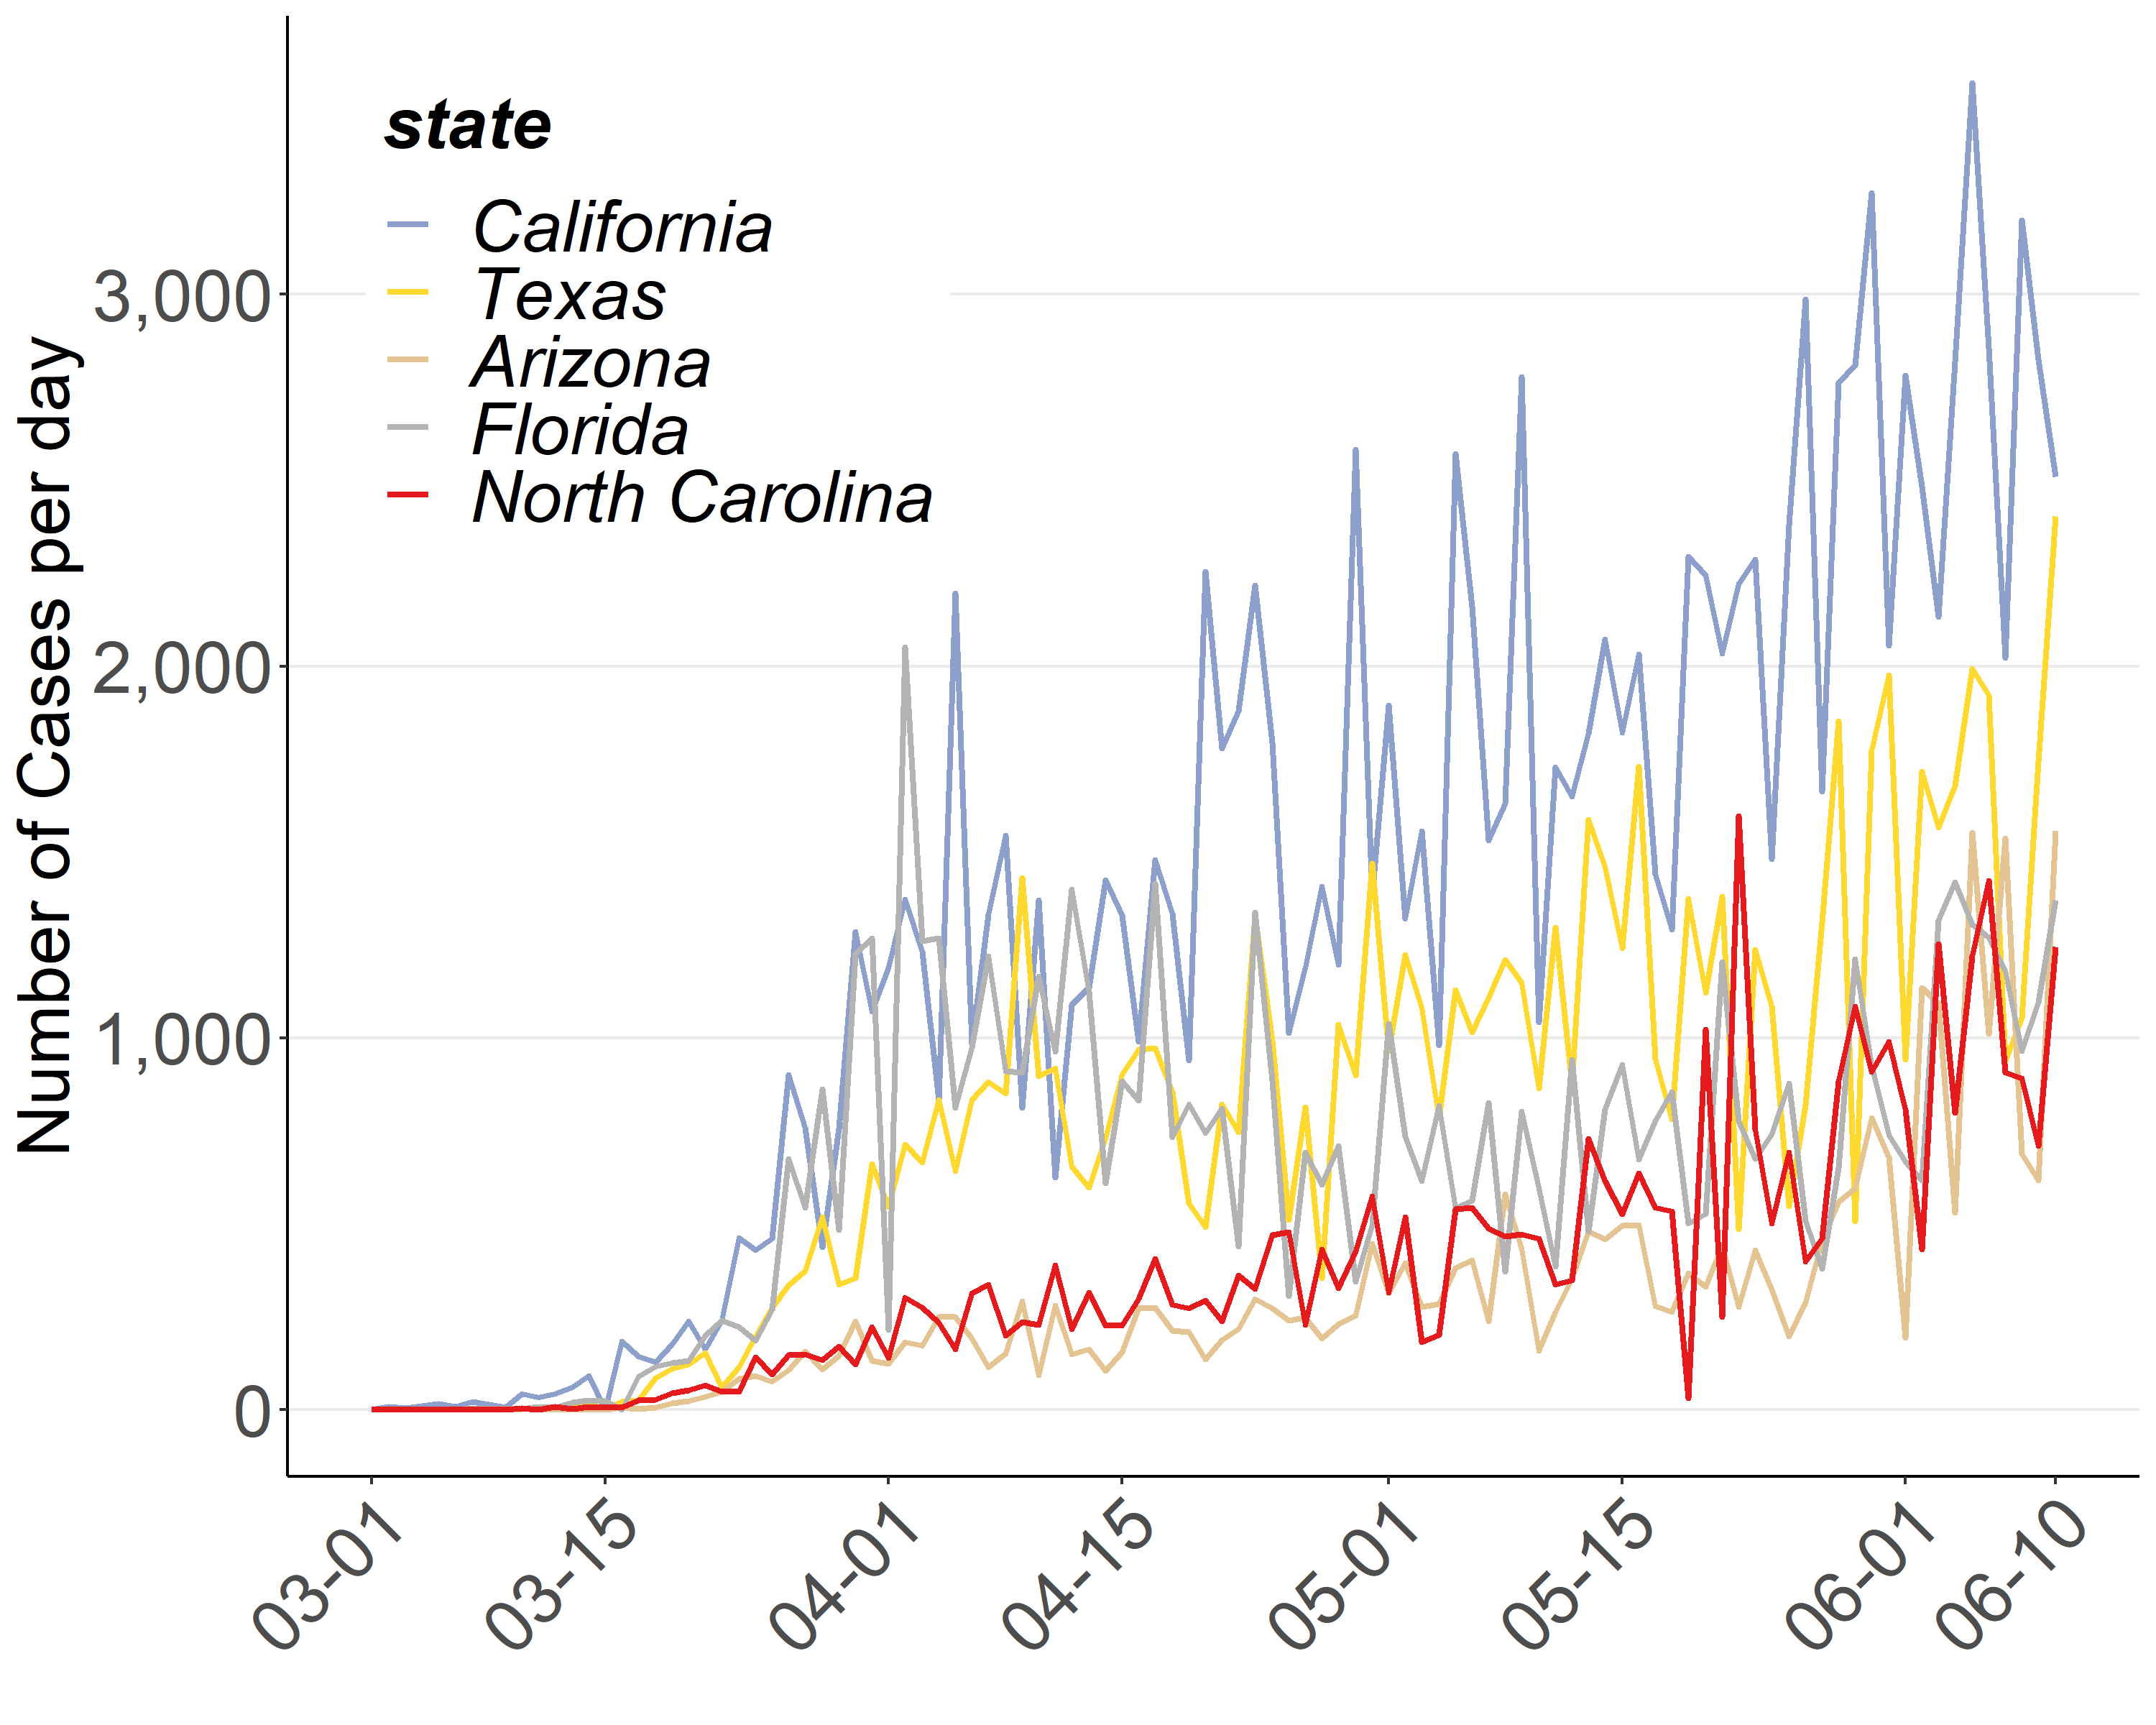
\includegraphics[]{./input/covid5.png}
\end{figure}

\begin{figure}[H]
\centering
\captionsetup{font={huge}}
\caption{美国日新增死亡前五位州趋势图}
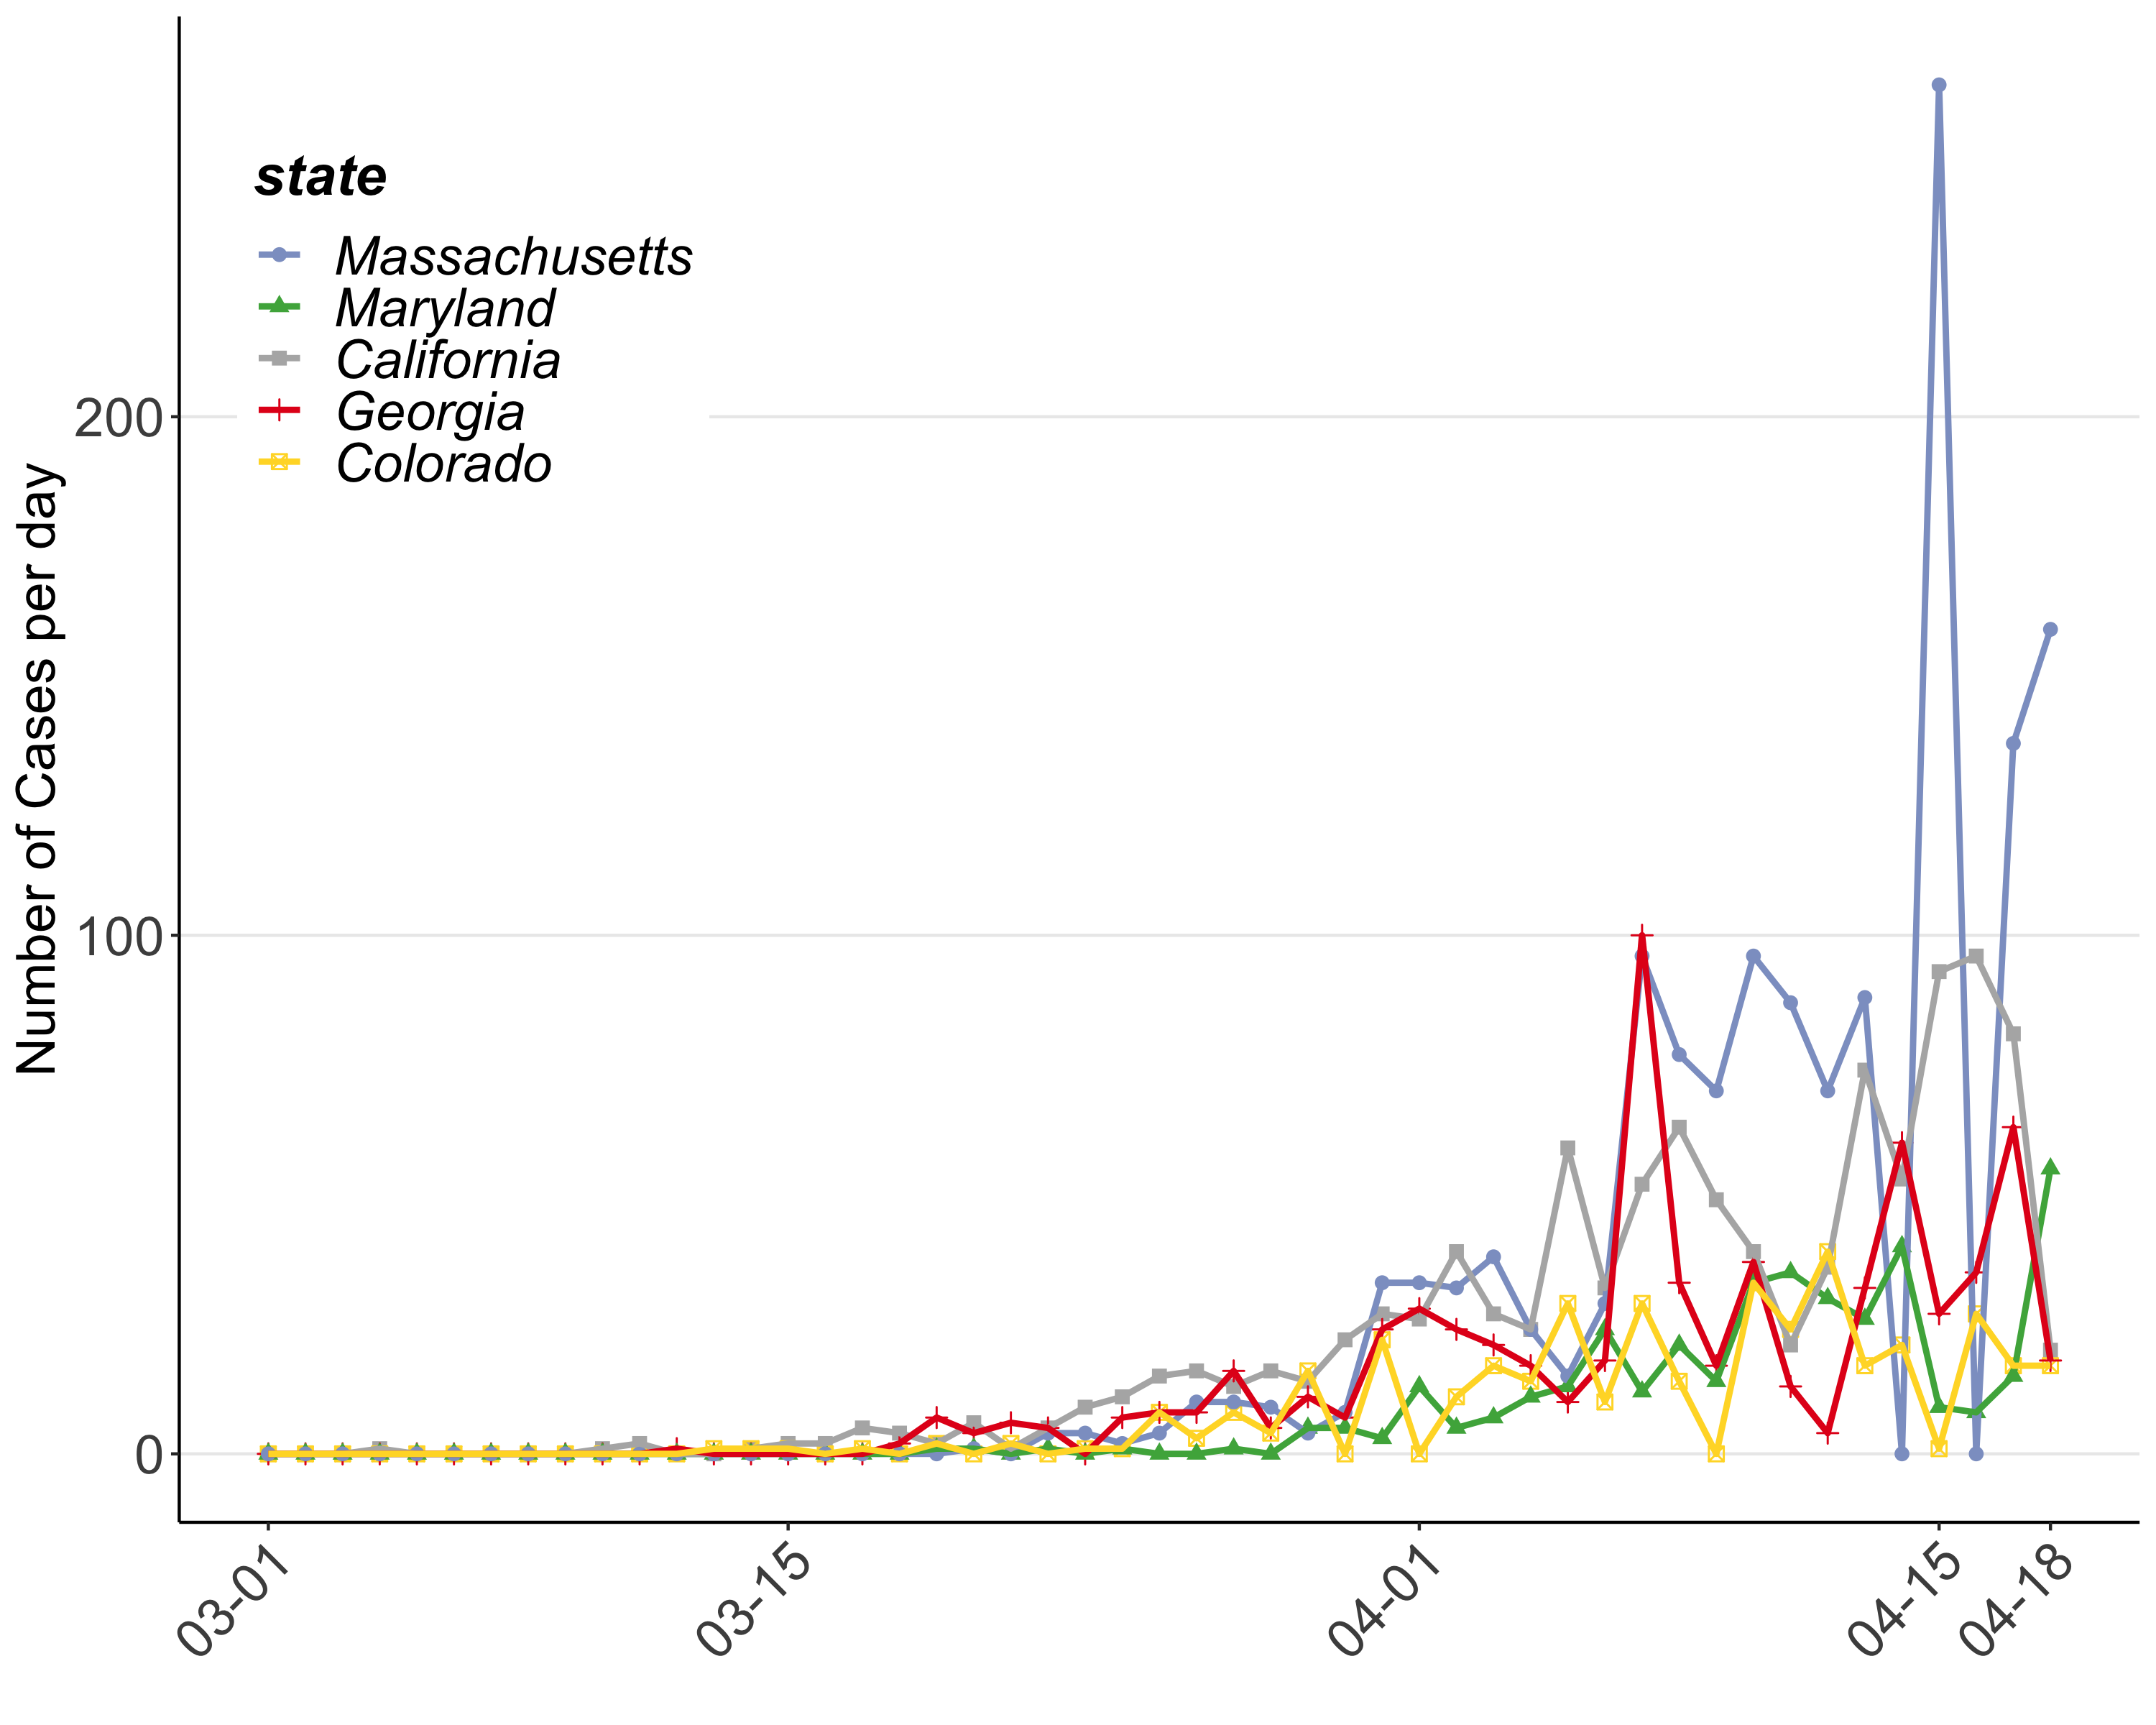
\includegraphics[]{./input/covid6.png}
\end{figure}

\begin{table}[H]
    \centering \begin{table}[H]
\centering\begingroup\fontsize{20}{22}\selectfont

\resizebox{\linewidth}{!}{
\begin{tabular}{rlrr}
\toprule
\multicolumn{0}{c}{\textbf{ }} & \multicolumn{3}{c}{\textbf{表3 美国新增确诊前十位州}} \\
  & 国家/州名 & 当日新增 & 累计确诊\\
\midrule
\rowcolor{gray!6}   & 美国 US & 58,114 & 3,363,056\\
1 & 佛罗里达州 FL & 12,624 & 282,435\\
\rowcolor{gray!6}  2 & 加利福尼亚州 CA & 8,814 & 333,357\\
3 & 得克萨斯州 TX & 7,016 & 269,778\\
\rowcolor{gray!6}  4 & 乔治亚州 GA & 3,637 & 120,572\\
5 & 田纳西州 TN & 3,314 & 65,274\\
\rowcolor{gray!6}  6 & 阿拉巴马州 AL & 1,958 & 55,545\\
7 & 北卡罗莱纳州 NC & 1,898 & 87,669\\
\rowcolor{gray!6}  8 & 路易斯安那州 LA & 1,705 & 79,827\\
9 & 南卡罗来纳州 SC & 1,520 & 58,168\\
\rowcolor{gray!6}  10 & 亚利桑那州 AZ & 1,357 & 123,824\\
\bottomrule
\end{tabular}}
\endgroup{}
\end{table} \end{table}\begin{table}[H]
    \centering \begin{table}[H]
\centering\begingroup\fontsize{20}{22}\selectfont

\resizebox{\linewidth}{!}{
\begin{tabular}{rlrrr}
\toprule
\multicolumn{0}{c}{\textbf{ }} & \multicolumn{4}{c}{\textbf{表4 美国新增死亡前十位州}} \\
  & 国家/州名 & 当日新增 & 累计死亡 & 病死率\%\\
\midrule
\rowcolor{gray!6}   & 美国 US & 400 & 135,605 & 4.0\\
1 & 得克萨斯州 TX & 60 & 3,276 & 1.2\\
\rowcolor{gray!6}  2 & 纽约州 NY & 45 & 32,395 & 8.1\\
3 & 加利福尼亚州 CA & 38 & 7,089 & 2.1\\
\rowcolor{gray!6}  4 & 佛罗里达州 FL & 35 & 4,277 & 1.5\\
5 & 新泽西州 NJ & 35 & 15,560 & 8.9\\
\rowcolor{gray!6}  6 & 康涅狄格州 CT & 23 & 4,371 & 9.2\\
7 & 乔治亚州 GA & 23 & 3,026 & 2.5\\
\rowcolor{gray!6}  8 & 密苏里州 MO & 13 & 1,105 & 3.9\\
9 & 南卡罗来纳州 SC & 11 & 972 & 1.7\\
\rowcolor{gray!6}  10 & 亚利桑那州 AZ & 9 & 2,246 & 1.8\\
\bottomrule
\end{tabular}}
\endgroup{}
\end{table} \begin{tablenotes}
        \fontsize{15}{15}
        \selectfont
        \item
      \end{tablenotes}
\end{table}

\(\bullet\)美国昨日新增确诊58,114例,新增死亡400例(表3和表4)。单日新增确诊排名前十位的州昨日新增均超过1,000例。

\(\quad\)\(\diamond\)佛罗里达州日新增确诊病例持续增长,近四日一直位于该国家日新增第一。

\(\quad\)\(\diamond\)纽约州昨日日新增死亡病例突增,近一周来首次成为该国家日新增死亡数第二。

\vspace{15mm}

\centering
\fontsize{12}{12}
\selectfont
\begin{tabular}{ll}


主编:马晶  &  副主编:仁晖,史珂玮 \\
责任编辑: 王雅晨 & 新闻组: 王宇 \\
数据分析:宋琰  & 微信排版:韩佩瑾 \\
\multicolumn{2}{l}{可视化组:张祺珉\, 刘逸洋\, 周梓淇\, 孙昊\, 唐星鸿\, 齐维为\,张立达}

\end{tabular}

\end{document}
